
\section{Background}
\label{sec:background}

\subsection{Blackjack Domain}

The objective of Blackjack is to obtain a higher number of points than the dealer without exceeding 21, where points are determined by cards held. Cards numbered 2 through 10 are worth their face value; face cards (Jack, Queen, King) are worth 10 points each; and aces are worth either 1 or 11 points. Our game consists of one player, the dealer, and one 52-card deck, shuffled prior to each game. The player bets \$1 prior to each hand, and the player and dealer are dealt two cards each, where only the value of the dealer's first card is known to the player. The player can then choose to either hit, which entails being dealt an additional card, or stand with the current hand, ending the player's turn. If the player exceeds 21, the game is over and the dealer wins the player's \$1. If not, the dealer hits until her points reach 17 or greater, in which case she must stand. \\

\noindent Blackjack players evaluate their hand relative to the dealer's card, often assuming that the dealer's hidden card is of value 10 \cite{b}. Since cards of value 10 account for 30 percent of cards in a 52 card deck, a plurality, they are the most likely point value for the dealer to hold. Such an assumption gives an approximate upper bound for the dealer's point total and is therefore a useful assumption to roughly estimate the actual state of the game. For instance, typical Blackjack wisdom holds that players ought to stand if the dealer shows a 6 and the player has some point total above 11. Since the dealer is likely to have 16 total points, she is likely to bust once she hits (which the dealer must do at sixteen). We explore the impact of the 10 point assumption in this paper. 

% 30 percent of cards in a 52-card deck are of point value 10, so we assume that the dealer's hidden card is always of value ten. This approach, therefore, represents the worst case scenario for  


% Since the dealer's second card is unknown to the player, she assumes that the dealer's points are their first card's value plus ten .

% (MAYBE THIS SHOULD GO IN Q LEARNING SINCE IT IS UNIQUE TO THAT????? - not really unique to Q learning but a relatively typical way to think about blackjack). Actually, I think maybe it should go in Q-learning since its not a proper part of the game but rather an assumption our player uses. 




% Describe any background information that the reader would need to know
% to understand your work. You do not have to explain algorithms or
% ideas that we have seen in class. Rather, use this section to describe
% techniques that you found elsewhere in the course of your research,
% that you have decided to bring to bear on the problem at hand. Don't
% go overboard here --- if what you're doing is quite detailed, it's
% often more helpful to give a sketch of the big ideas of the approaches
% that you will be using. You can then say something like ``the reader
% is referred to X for a more in-depth description of...'', and include
% a citation.\\

% This section is also a good place to describe any data pre-processing
% or feature engineering you may have performed. If you are \emph{only}
% discussing data wrangling in this section, it's recommended that you
% amend the title of the section to ``Data Preparation'' or something
% similar; otherwise, use subsections to better organize the flow.

\subsection{Q-Learning}
Q-learning is a model-free reinforcement learning algorithm. More specifically, Q-learning is a temporal difference algorithm which directly approximates the optimal state-action value function $Q^* (s,a)$, which is defined as the expected sum of discounted future rewards assuming that the agent takes action $a$ in state $s$, acting optimally in each later state \cite{rn}. The optimal state-action value function is obtained by updating the state-action value function $Q(s,a)$ episodically, so in Blackjack, $Q(s,a)$ is updated after each game. The optimal policy is that which maximizes rewards over time. De Granville provides the following pseudocode for the Q-learning algorithm: \\ 

    \noindent Initialize $Q(s,a)$ arbitrarily \\
    
    \noindent For each episode: \
    
        Choose $a$ from $s$ using policy derived from $Q$ \
        
        Take action $a$, observe reward $r$, and new state $s'$ \
        
        $Q(s,a) = Q(s,a) + \alpha[r + \gamma \text{ max}_{a'} Q(s',a') - Q(s,a)]$ \
        
        $s = s'$ \
        
    \noindent until $s$ is terminal \\

\noindent Note that $\alpha$ refers to the learning rate, which determines the size of the update made each episode, and $\gamma$ is the discount rate, which determines the weight of future rewards \cite{q}. For selecting an action to take from a given state, many Q-learning algorithms use the epsilon-greedy strategy. This strategy introduces randomness to the selection of actions which allows the algorithm to better train the policies and avoid local minima. \\

\noindent If each state-action pair is continually updated, Q-learning is expected to converge to the optimal state-action value function with probability 1 \cite{q}. Because Q-learning begins with an arbitrary model, it is expected to perform similarly to the random player at first. It should subsequently tend towards the performance of the heuristic player as it learns, developing a policy which approaches optimality. 


\subsection{Other Policies}
In order to evaluate the success of our Q-learning algorithm, we compare its results to that of a random player and a heuristic player, which utilizes a basic, static policy. 

\begin{itemize}
    \item \textbf{Random Player}: randomly chooses an action, either hit or stand, at each given state where each action has an equal probability of being chosen. 
    \item \textbf{Heuristic Player}: leverages a near-optimal static policy proposed by Howard \cite{o}. The policy is given by the following set of rules: \ 
    
    \begin{figure}[htb]
      \centering  % centers the image in the column
      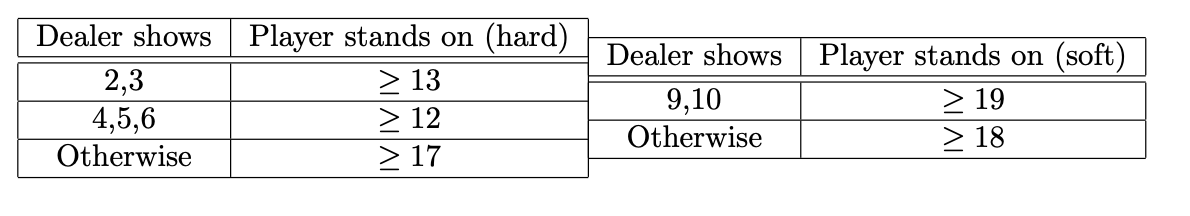
\includegraphics[width = 3.4in]{a.png} 
      % *Every* figure should have a descriptive caption.
      \caption{Static Blackjack policy. Image courtesy of \texttt{Howard $2016$}.}
     \label{fig:tex}

    \end{figure}
\end{itemize}
\noindent We call the heuristic policy static since the player adheres to the strict set of rules in order to make decisions at each given state. A typical optimal policy gives the player a 4 percent disadvantage, so we consider this policy near optimal. \\

\noindent The random and heuristic players set realistic lower and upper bounds, respectively, on the performance of our player. Our goal for the Q-learning algorithm was to devise a policy which tends towards, and ideally would exceed, the performance of the heuristic policy. 



